
\section{RFID Intro}
\begin{tabular}[h]{c c}

\parbox{6cm}{
    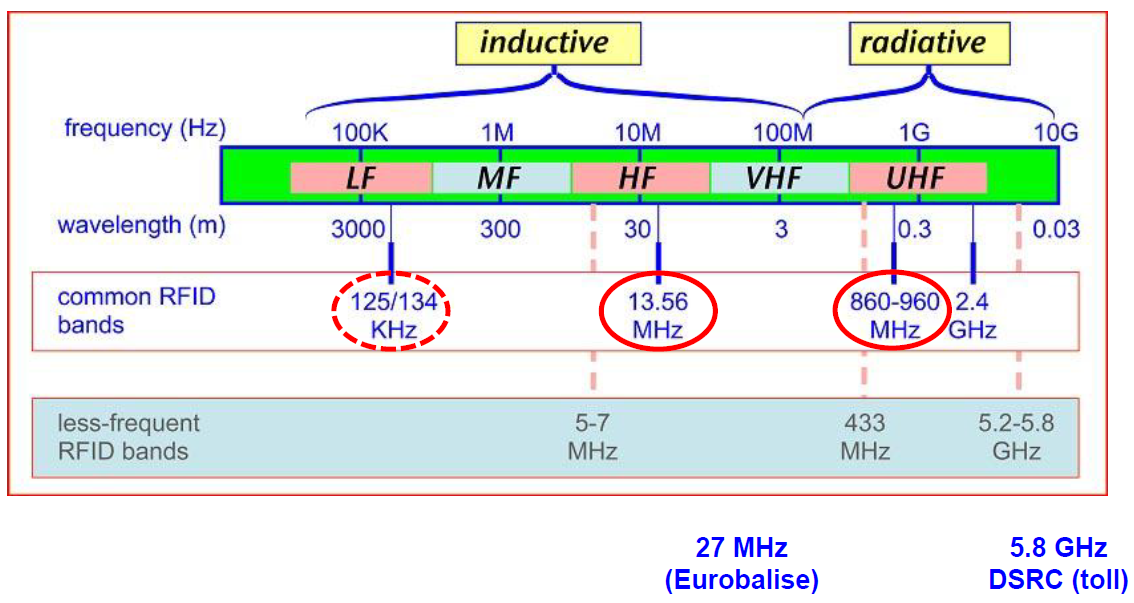
\includegraphics[width=8cm]{./bilder/RFIDFrequenzen.png} } 
&

\parbox{6cm}{
    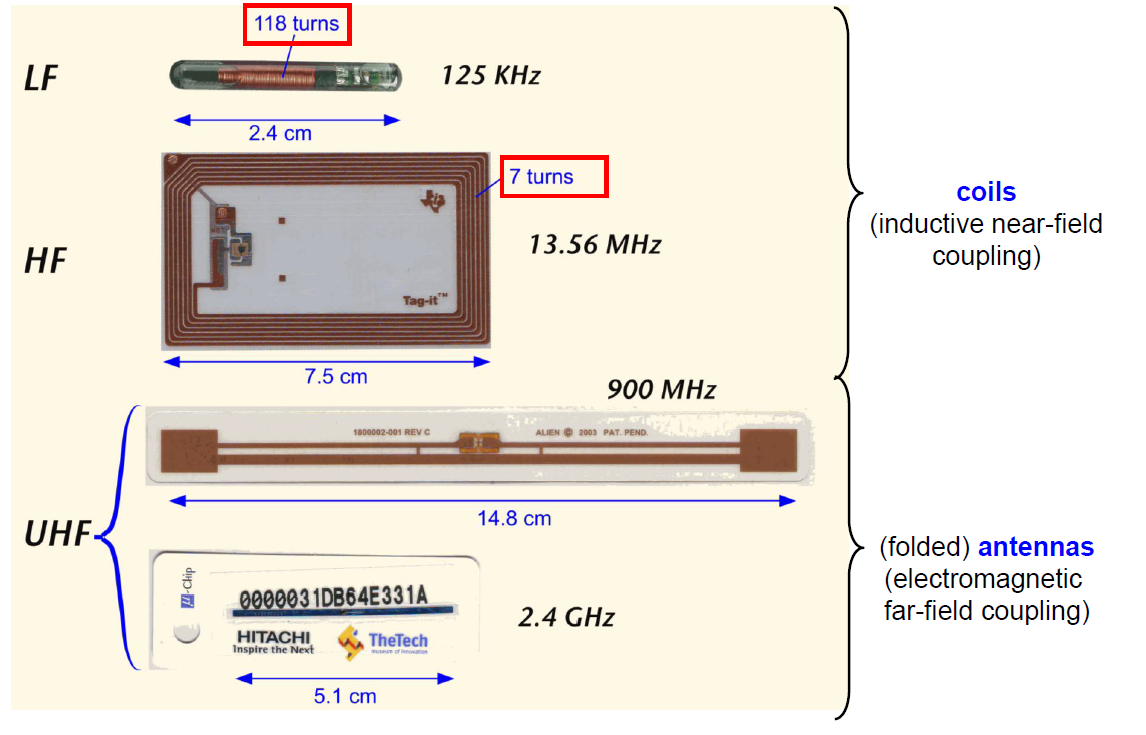
\includegraphics[width=8cm]{./bilder/RFIDTags.png} } \\
\end{tabular}
\subsection{Aktiv vs. Passiv}
	\begin{itemize}
		\item Passiv: Ich sende und empfange gleichzeitig, Frequenzen müssen leicht verschoben sein
		\item Semi-Passiv: Ich kann NICHT antowrten, wenn ich angestrahlt werden. Ich habe Batterie für Tag Power. 
		\item Aktiv: Ich kann antworten auch wenn ich nicht angestrahlt werde. ich habe Batterie für Tag und Radio. 
	\end{itemize}
\subsection{Antikollisionsprotokolle}
	\begin{itemize}
		 \item Deterministisches Antikollisionsprotokoll: Baumsuche anhand von ID (und Maske). Leserate: 10-30 Tags/s
		 \item Probabilistisches Antikollisionsprotokoll: Modifiziertes Aloha Protokoll (mit Random Nr). Leserate. 100-500 Tags/s
	\end{itemize}
\section{RFID HF}
	\begin{itemize}
		\item Hohe Frequenz $\rightarrow$ 3-10 Windungen
		\item Tiefe Frequenz $\rightarrow$ 100-1000 Windungen
		\item Spulengrösse $\rightarrow$ Leseabstand = Spulendurchmesser
	\end{itemize}
\subsection{Modulation}
	\begin{itemize}
		\item Reader -> Tag: ASK Modulation, Nicht zu viele Nullen senden, sonst hat Tag zu wenig Power. Je höher Modulationstiefe, umso weniger Energie. 
		\item Tag -> Reader: Lastmodulation, Manchester coded, Tag schliesst Antenne kurz, wird auf Hauptträger draufmoduliert (mit Subträger)
	\end{itemize}
\subsection{Standards}
	\begin{itemize}
		\item LF
			\begin{itemize}
				\item ISO/IEC 11784/5 and extension 14223 identification of animals
			\end{itemize} 
		\item HF
			\begin{itemize}
				\item ISO/IEC 14443
				Identification Cards – Proximity Cards (2001) range up to 10 cm, data rate 106 kb/s
				\item SO/IEC 15693
				Identification Cards– Vicinity Cards (2001), range up to 1m, data rate 26kb/s, ISO/IEC 18000 - 3 mode1, 20Tags/s
				\item ISO/IEC 18000-3 mode 3(item management standard), HF-version of EPC UHF Gen2, high data and high reading rates, 300Tags/s
				
				
				
			\end{itemize}
	\end{itemize}
\section{RFID UHF}
